\chapter{UTILIZAREA APLICAȚIEI}

\section{Instalarea aplicației}

Pentru a putea folosi aplicația trebuie să fie instalate mai multe componente:
\begin{itemize}
    \item \textit{Docker} - pentru storage
    \item \textit{dotnet tool} - pentru comenzi în terminal și compilarea .NET;
    \item \textit{Azurite} - emulatorul pentru Azure Storage;
    \item \textit{SignalR Emulator} - emulatorul pentru server-ul SignalR;
    \item \textit{Azure Functions Tools} - pentru pornirea proiectului Azure;
    \item \textit{ngrok/Visual Studio sau Rider} - în caz de deployment sau doar un IDE pentru rularea codului.
\end{itemize}

Prima dată se obține codul, fie din surse, fie de pe GitHub.

Trebuie instalat \textit{Docker} deoarece \textit{Azurite} vine cu foarte multe fișiere temporale și
există riscul ca mașina să rămână fără memorie.

Următorul pas reprezintă deschiderea unui \textit{Terminal}, și să se navigheze către folderul \textit{Docker} din proiect, folosind
comanda:
\begin{verbatim}
    cd C:\Work\FastRide\fast-ride\Run\Docker
\end{verbatim}
Apoi trebuie rulată următoarea comadă pentru a instala \textit{Azurite}:
\begin{verbatim}
    docker-compose up -d
\end{verbatim}
Dacă există eroare privind comanda \textit{docker-compose}, atunci acesta trebuie instalat.
Urmează să se instaleze \textit{dotnet tool} și să se instaleze \textit{SignalR Emulator}-ul prin comanda:
\begin{verbatim}
    dotnet tool install -g Microsoft.Azure.SignalR.Emulator
\end{verbatim}

Mai departe trebuie deschis \textit{Docker}-ul și pornit \textit{Azurite}, apoi rularea comenzii:

\begin{verbatim}
    cd C:\Work\FastRide\fast-ride\Run\Docker
    asrs-emulator start
\end{verbatim}

Pentru a rula codul, fie se deschide un IDE cu ambele soluții și se rulează, fie se rulează din terminal
cu beneficiul de a publica în rețea aplicația. Pentru terminal trebuie rulate următoarele comenzi:

\begin{verbatim}
    cd C:\Work\FastRide\fast-ride\FastRide.Server
    func start

    ngrok http http://localhost:7102 # pentru ngrok (din ngrok.exe)
\end{verbatim}

Dacă se folosește \textit{ngrok} atunci trebui actualizată configurația din Client pentru \textit{SDK}-ul server-ului.
\begin{verbatim}
    cd C:\Work\FastRide\fast-ride\FastRide.Client
    dotnet run --urls "http://localhost:7028"
    ngrok http https://localhost:7028 # pentru ngrok (din ngrok.exe)
\end{verbatim}


\section{Manual de utilizare}

Aplicația FastRide este concepută pentru a facilita rezervarea și acceptarea curselor între
clienți și șoferi într-un mod rapid, sigur și intuitiv. Utilizatorul se autentifică
cu un cont Google, își poate introduce un număr de telefon (dacă nu a fost deja 
preluat automat) și poate începe imediat să interacționeze cu platforma.
Clienții pot vizualiza harta, alege punctul de plecare și destinația, iar aplicația
va calcula ruta și va căuta șoferi disponibili în apropiere. Odată ce un șofer 
acceptă cursa, aceasta devine activă și poate fi urmărită în timp real. La final, 
clientul poate oferi un rating, iar istoricul curselor este salvat pentru consultare 
ulterioară.

Diagrama \textit{Use Case} reflectă interacțiunile principale dintre utilizatori și sistem. 
Există trei tipuri de actori: clientul (\textit{User}), șoferul (\textit{Driver}) și administratorul (\textit{Admin}).
Clientul poate efectua acțiuni precum: 
autentificare, rezervare cursă, vizualizare rută, urmărire în timp real și acordare de rating. 
Șoferul, la rândul său, se autentifică, primește 
notificări cu cereri de curse, le poate accepta, vede traseul și finalizează cursa. Iar administratorul, în plus,
poate să asigneze roluri utilizatorilor. 
Toate aceste interacțiuni sunt coordonate de sistemul backend, care se ocupă de procesarea 
cererilor, actualizarea în timp real a stărilor și salvarea datelor în storage.

În analiza cazurilor de utilizare, diagrama \textit{Use Case} nu doar conturează 
funcționalitățile sistemului, ci evidențiază și relațiile de dependență între acțiuni 
și actori. Un aspect important vizibil în diagramă este separarea clară a 
responsabilităților, ceea ce permite o arhitectură ușor de întreținut. 
De exemplu, legătura dintre client și acțiunea de evaluare a șoferului apare doar 
după încheierea unei curse, ceea ce indică un flux condiționat logic. Similar, 
interacțiunea șoferului cu cursa, este posibilă doar în momentul în care aceasta a 
fost creată și nu este deja acceptată, ceea ce reflectă restricții de business 
transpuse clar în comportamentul aplicației. În acest fel, diagrama devine nu doar o 
hartă a funcționalităților, ci și o expresie a regulilor din spatele aplicației.

\begin{figure}[H]
    \centering
    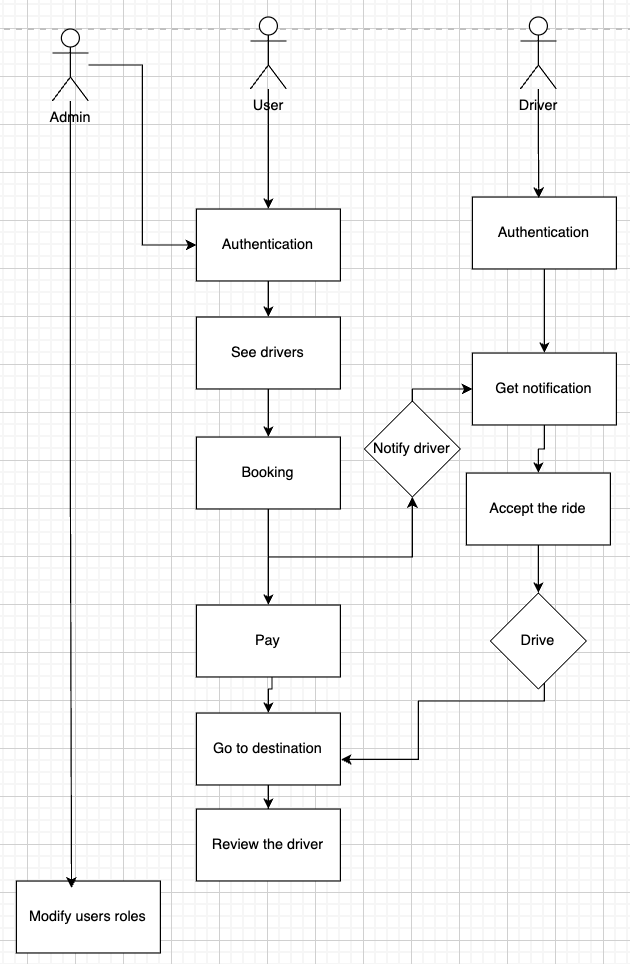
\includegraphics[width=15cm]{Assets/UserCase.png}
    \caption{Diagrama \textit{Use case} a proiectului.}
    \label{fig:UserCase}
\end{figure}

Aplicația este \textit{responsive} și este suportată atât pe desktop cât și pe mobile.

\begin{figure}[H]
    \centering
    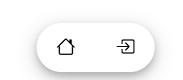
\includegraphics[width=4cm]{Assets/responsive1.png}
    
\includegraphics[width=10cm]{Assets/responsive2.png}
    \caption{Bara de navigare pe desktop și mobile.}
    \label{fig:responsive}
\end{figure}

\subsection{Experiența utilizatorului}

Utilizatorul trebuie să se autentifice în aplicație, prin contul Google, apăsând butonul de \textit{login}. 
Această etapă este necesară pentru a putea accesa funcționalitățile aplicației.
Fără autentificare, utilizatorul poate doar să vadă locația curentă și să
caute diverse locații pe hartă.

\begin{figure}[H]
    \centering
    
\includegraphics[width=1cm]{Assets/human.png}
    \caption{Mark-ul \textit{human} ce indică locația actuală a utilizatorului.}
    \label{fig:humanMark}
\end{figure}

După autentificare, utilizatorul își poate rezerva o cursă. Acest lucru se realizează prin
plasarea unui \textit{pin} pe hartă, ce indică locul unde dorește să fie lăsat.

\begin{figure}[H]
    \centering
    
\includegraphics[width=1cm]{Assets/pin.png}
    \caption{Mark-ul \textit{pin} pentru a sugera destinația.}
    \label{fig:pinMark}
\end{figure}

Pentru a realiza acest lucru, fie se face click pe hartă, fie se folosește bara de search cu sugestii.

\begin{figure}[H]
    \centering
    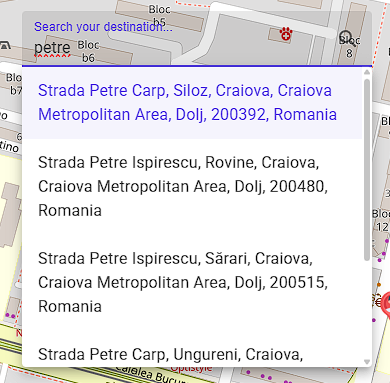
\includegraphics[width=8cm]{Assets/search.png}
    \caption{Bara de căutare pentru adrese cu sugestii.}
    \label{fig:searchAddress}
\end{figure}

Utilizatorul poate apăsa butonul \textit{Ride} pentru a porni cursa.
Pe hartă se afisează și ceilalți șoferi ce sunt disponibili pentru a accepta o cursă din aceiași localitate.

\begin{figure}[H]
    \centering
    
\includegraphics[width=1cm]{Assets/driver.png}
    \caption{Mark-ul \textit{driver} ce semnifică un utilizator de tip șofer disponibil.}
    \label{fig:driverPin}
\end{figure}

Odată apăsat butonul, utilizatorul trebui sa treacă prin doi pași: să confirme cursa și să ofere informații despre cardul bancar. 
După apăsarea butonului și pregătirea cursei în server, un pop-up 
cu toți pașii i se deschide și trebuie completat. Dacă ceva nu este în ordine, utilizatorul primește
feedback în legătura cu erorile.

\begin{figure}[H]
    \centering
    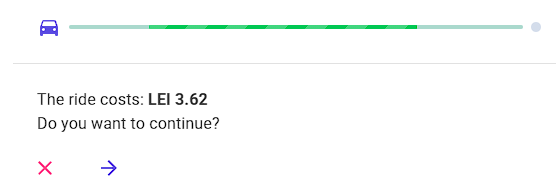
\includegraphics[width=14cm]{Assets/acceptRideUser.png}
    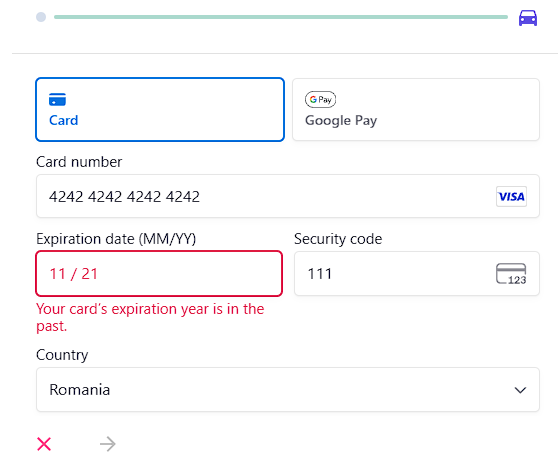
\includegraphics[width=14cm]{Assets/card.png}
    \caption{Pașii pe care utilizatorul trebuie să îi completeze.}
    \label{fig:paymentStep12}
\end{figure}

\begin{figure}[H]
    \centering
    
\includegraphics[width=14cm]{Assets/donePayment.png}
    \caption{Mesajul de confirmare că totul este în regulă.}
    \label{fig:paymentStep3}
\end{figure}

Mai departe, utilizatorul așteaptă pentru ca un șofer să îi accepte cursa. În caz că nu se găsește un șofer atunci cursa este anulată.
Fiecare status de anulare se observă în meniul de informare, ce ține locul bării de căutare.

\begin{figure}[H]
    \centering
    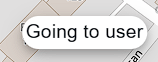
\includegraphics[width=7cm]{Assets/status.png}
    \caption{Meniul de informare al status-ului.}
    \label{fig:statusMenu}
\end{figure}

Dacă s-a găsit un șofer, atunci utilizatorului i se deschide un pop-up cu detaliile
despre acesta și apoi este nevoie să aștepte ca șoferul să ajungă să îl preia. După ce clientul se află în mașina șoferului, pot să meargă împreună spre 
destinație.

\begin{figure}[H]
    \centering
    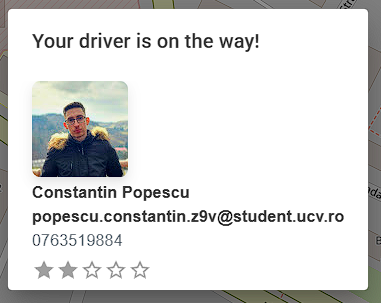
\includegraphics[width=10cm]{Assets/driverDetails.png}
    \caption{Detaliile despre șofer după ce acceptă cursa.}
    \label{fig:driverDetails}
\end{figure}

Utilizatorul poate vedea ruta pe unde șoferul o să meargă, iar \textit{pin}-ul ce indică
locația curentă se modifică în \textit{currentCar}.

\begin{figure}[H]
    \centering
    
\includegraphics[width=1cm]{Assets/currentCar.png}
    \caption{Mark-ul \textit{currentCar} ce semnifică că utilizatorul călătorește cu mașina.}
    \label{fig:currentCar}
\end{figure}

La final de cursă, opțional, clientul poate lăsa o recenzie șoferului.

\begin{figure}[H]
    \centering
    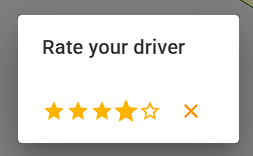
\includegraphics[width=6cm]{Assets/rateDriver.png}
    \caption{Dialog-ul ce permite oferirea unui recenzii șoferului.}
    \label{fig:rateDriver}
\end{figure}

Alte lucruri pe care le poate face clientul, dar și celelalte tipuri de utilizatori,
este să își schimbe numărul de telefon sau să navigheze către Google Accounts pentru a își schimba numele sau imaginea de profil.

\begin{figure}[H]
    \centering
    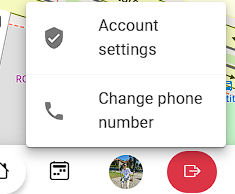
\includegraphics[width=7cm]{Assets/popoverUser.png}
    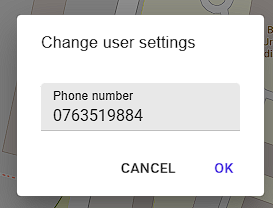
\includegraphics[width=8cm]{Assets/changePhoneNumber.png}
    \caption{Schimbarea numărului de telefon apăsând pe imaginea de profil.}
    \label{fig:phoneNumberChange}
\end{figure}

Utilizatorii pot vedea și istoricul curselor prin apăsarea butonului din bara de navigare.
Pentru fiecare cursă se poate vedea adresa de destinație, data și ora la care s-a completat cursa, prețul plătit
și, în cazul de anulare a cursei, motivul anulării. Folosind butonul \textit{Rebook}, utilizatorul poate
să repună \textit{pin}-ul în același loc precum în istoric.

\begin{figure}[H]
    \centering
    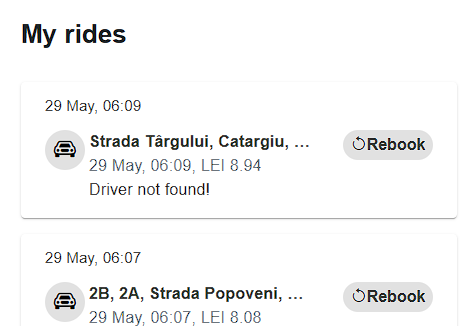
\includegraphics[width=10cm]{Assets/history.png}
    \caption{Istoricul curselor.}
    \label{fig:historyRides}
\end{figure}

\subsection{Experiența șoferului}

Șoferul nu are accesul să rezerve o cursă, însă este asignat să accepte una, de aceea flow-ul acestuia începe după 
ce un client începe o cursă și îi se atribuie cererea. Bineînțeles, trebuie să fie autentificat.

El are un alt buton, \textit{GetRides} care deschide un dialog unde poate vedea cursele asignate ce i sunt asignate.

\begin{figure}[H]
    \centering
    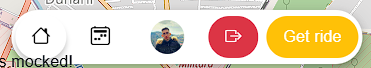
\includegraphics[width=8cm]{Assets/driverNavBar.png}
    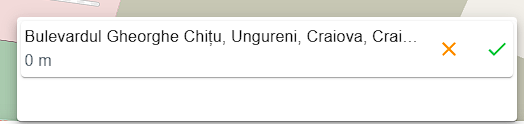
\includegraphics[width=10cm]{Assets/acceptRide.png}
    \caption{Bara de navigare împreună cu dialogul-ul ce afișează ofertele curente.}
    \label{fig:driverNavBar}
\end{figure}

Singura responsabilitate a șoferului, după ce a acceptat cursa, este să meargă la client, să îl aștepte și să
meargă împreună spre destianție. În acești pași, șoferul are prima destinație către client, apoi către destinația propiu zisă.

Ca și ajutor în trafic, acesta poate să vadă ruta spre punctul de destinație, actualizându-se în timp real și poate regăsi și
indicații de navigare.

\begin{figure}[H]
    \centering
    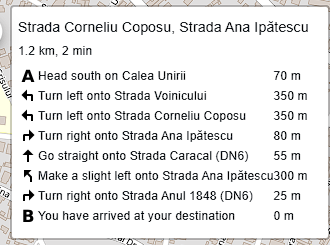
\includegraphics[width=10cm]{Assets/indicates.png}
    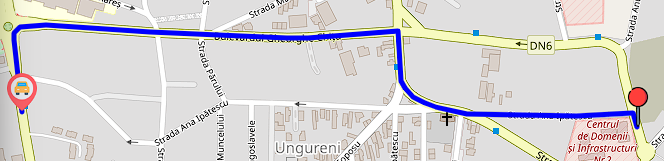
\includegraphics[width=10cm]{Assets/route.png}
    \caption{Exemplu de rută și indicații de navigare.}
    \label{fig:indicates}
\end{figure}

\subsection{Experiența admin-ului}

În plus de cele menționare la utilizatorul normal, administratorul poate schimba tipul 
oricărui utilizator, iar, de asemenea, mai poate actualiza și numărul de telefon.
Prin apăsarea butonul din bara de navigare, i se deschide un tabel unde poate vedea toate informațiile despre utilizatori.
El poate să-și filtreze utilizatorii după numărul de telefon, nume, email sau identificator.
\begin{figure}[H]
    \centering
    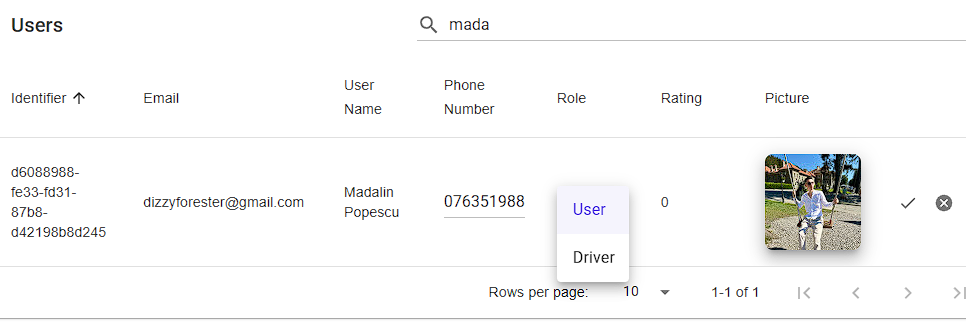
\includegraphics[width=16cm]{Assets/adminPage.png}
    \caption{Pagina administratorului.}
    \label{fig:adminPage}
\end{figure}

Aplicația FastRide oferă o experiență intuitivă și eficientă pentru utilizatorii 
care doresc să rezerve sau să accepte curse într-un sistem de ride-sharing. 
Printr-un proces simplificat de autentificare cu contul Google, utilizatorii pot accesa
rapid funcționalitățile esențiale, precum vizualizarea hărții, stabilirea destinației, comunicarea în timp real și evaluarea curselor. 
Interfața este ușor de folosit, iar integrarea serviciilor externe precum Stripe, 
SignalR și Leaflet contribuie la o funcționare fluidă și sigură, atât pentru clienți, 
cât și pentru șoferi.